%!TEX program=luatex

\newpage

\section{Introduction}
Les systèmes de recommandation demeurent aujourd'hui un moyen non négligeable pour l'amélioration de l’expérience utilisateur sur les réseaux sociaux, le e-commerce et sur les moteurs de recherche.\\
Ces derniers contribuent d'une manière considérable dans l'accroissement de plusieurs fermes technologiques tels que \emph{Facebook}, \emph{Amazon} ou \emph{Google} qui exploitent des quantités massives de données (Big data) afin de faire des recommandations avec un niveau de confiance assez élevé.\\
Il sera question, dans ce chapitre, d’effectuer une description de l'état de l'art par la présentation des systèmes de recommandations et leurs utilisations, une brève présentation de l'apprentissage automatique et ces différentes techniques, et nous allons conclure par l'introduction des techniques de profilage d'utilisateurs et de la prédiction des comportements.

\section{Apprentissage automatique}
\subsection{Définition}
\emph{L'apprentissage automatique} consiste à développer des programmes informatiques qui ont la capacité d’améliorer leur performances avec de l’expérience et de changer leurs comportement pour s'adapter à des besoins selon certains critères.\\
Souvent on a recours à l'apprentissage automatique lorsque on ignore le modèle adéquat à utiliser pour la résolution d'un problème donné, on peut citer aussi :
\begin{itemize}
    \item le manque d'expertise sur le problème.
    \item la difficulté et la complexité des solutions disponibles. 
    \item L'espace des solutions du problème est très grand et change dans le temps.\cite{guess} 
\end{itemize}

\subsection{Paradigmes de l'apprentissage automatique}
Dans le domaine de la \textbf{Data science} on peut trouver plusieurs algorithmes d'apprentissage automatique.\\Ces algorithmes peuvent être classés dans deux groupes basés sur la façon avec laquelle ils \emph{apprennent} à prédire : supervisé et non supervisé.

\subsubsection{Apprentissage automatique supervisé}
L'apprentissage supervisé est ainsi nommé car il nécessite l'intervention de l'être humain (souvent un expert) pour spécifier à l'algorithme les résultats qu'il devrait fournir.\\
L'apprentissage supervisé nécessite que les sorties possibles de l'algorithme soient déjà connues et que les données utilisées pour former l'algorithme soient déjà étiquetées avec des réponses correctes. Donc, les données d'apprentissage doivent être labellisées/classifiées au préalable en plus des caractéristique d'identification.\\
Le problème le plus traité est \textbf{la classification} qui consiste à identifier à quelle catégorie appartient un objet.\\
\begin{table}[H]
    \begin{center}
        \begin{tabular}{|c|c|c|c|}
            \hline
            \textbf{Sexe} & \textbf{Age}(ans) & \textbf{Poids}(kg) & \textbf{Diabétique}  \\
            \hline
            H  &  25 & 68  &  Non\\
            \hline
            F  &  50 & 75  &  Oui\\
            \hline
            H  &  38 & 85 &   Oui\\
            \hline
            F  &  75 & 60 &   Non\\
            \hline
            H  &  14 & 30  &  Non\\
            \hline
        \end{tabular}
    \end{center}
\caption{Une partie d'un dataset destiné à la classification}
\end{table}

\subsubsection{Apprentissage automatique non-supervisé}
L'apprentissage automatique non supervisé consiste à déduire une fonction à partir de données \textbf{non labellisées/étiquetées} en utilisant des algorithmes basés sur le calcul de la similarité entre ces données.\\
Les données seront divisé en sous-groupes de manière que ces derniers seront le plus possible similaires.
Ce type d'apprentissage est très utilisé dans le domaine de l'imagerie médical, la détection d'anomalie et la recommandation.\\
La technique la plus utilisée est \textbf{le clustering}, pour l'appliqué on s'appuie sur des algorithmes plus ou moins complexes, tels que les algorithmes des k-moyennes ou k-medoids.
\begin{table}[H]
    \begin{center}
        \begin{tabular}{|c|c|c|}
            \hline
            \textbf{Sexe} & \textbf{Age}(ans) & \textbf{Poids}(kg) \\
            \hline
            H  &  25 & 68 \\
            \hline
            F  &  50 & 75 \\
            \hline
            H  &  38 & 85 \\
            \hline
            F  &  75 & 60 \\
            \hline
            H  &  14 & 30 \\
            \hline
        \end{tabular}
    \end{center}
\caption{Une partie d'un dataset destiné au clustering}
\end{table}

\section{Les systèmes de recommandations}
\subsection{Définition}
Un système de recommandation est un mécanisme de filtrage de l'information qui permet de proposer à des utilisateurs des éléments qui sont susceptibles de les intéresser selon leurs préférences et leurs comportements.\\
Le but final est de prédire votre appréciation afin de vous suggérer des éléments similaires que vous êtes en mesure d'apprécier.\\
Ces systèmes utilisent des techniques très avancés de l'intelligence artificielle tels que l'apprentissage automatique, le traitement automatique de la langue et la recherche d'informations. 

\subsection{État de l'art}
Compte tenu de l'importance des systèmes de recommandation qui permettent de cibler l'utilisateur selon ses caractéristiques (profil), plusieurs modèle de ces derniers ont vue le jour. Nous allons expliciter quelques uns :

\subsubsection*{Système de recommandation pour les réseaux sociaux :}
\textbf{LinkedIn :} LinkedIn est un réseau social professionnel qui fait usage des systèmes de recommandation. Celui ci utilise un filtrage collaborative à base d'objets (Membre, Emploi, Société, Groupe) grâce à un module de recommandation disponible dans chaque profil permettant de recommander d'autres membres fréquemment associés au profil actuel ou du même groupe ou postulant pour le même emploi.\\
    \begin{figure}[H]
        \centering
            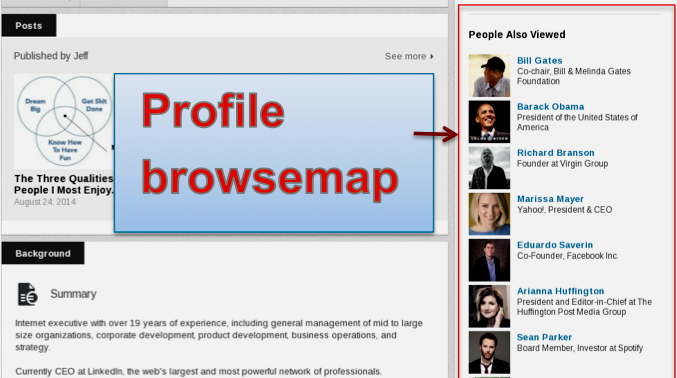
\includegraphics[height=150pt,width=300pt]{img/chapter1/linkedin.png}
        \caption{Recommandations sur le réseau social LinkedIn\cite{linkedin}}
    \end{figure}

\subsubsection*{Système de recommandation pour les Plate-forme de e-commerce :}
\textbf{Amazon :} Amazon est un site internet de vente en ligne, très répondu dans le monde, il compte des millions d'utilisateurs; pour cela, le développement d'un système de recommandation était une tache majeure. Les ingénieurs d'Amazon ont opté depuis le début pour une approche basé sur un \emph{filtrage collaboratif basé mémoire} (memory-based collaborative filtering) celui-ci permet de recommander les produits en se basant sur les produits préférés par les utilisateurs similaires mais aussi de cibler les produits similaires à ceux déjà achetés ou noté.\cite{amazon} Aujourd'hui, cette approche a permis de faire d'énorme gains économiques puisqu’elle représente à elle seule 35\% du chiffre d'affaire d'Amazon selon une étude de McKinsey's Chicago office.\\ 
    \begin{figure}[H]
        \centering
            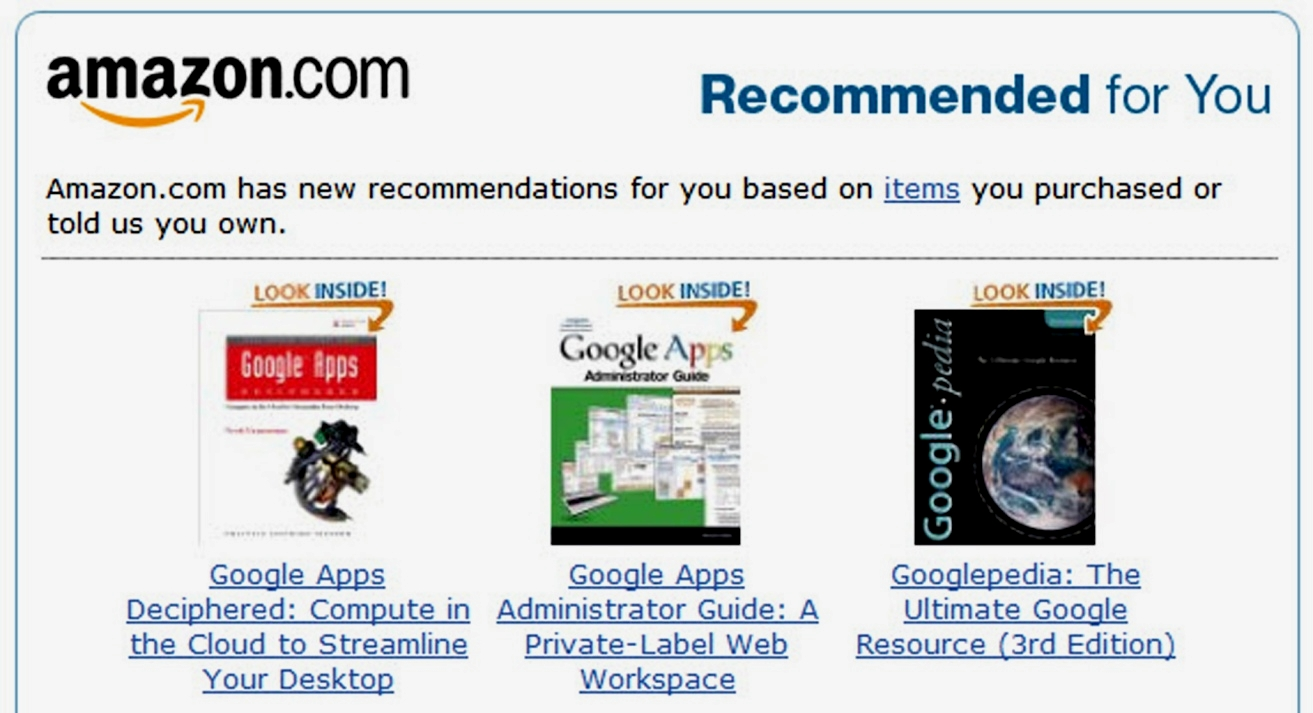
\includegraphics[height=150pt,width=300pt]{img/chapter1/amazon.jpg}
        \caption{Recommandations sur le site \emph{amazon.com}}
    \end{figure}

\subsubsection*{Système de recommandation pour les plate-forme de streaming vidéo :}
\textbf{Netflix :} Netflix est un média qui propose contenu vidéo (films, séries, documentaires...) en flux continu sur internet. Comme ce site est très prisés partout dans le monde, Netflix se concentre beaucoup sur les systèmes de recommandation pour proposer les vidéos appropriés aux utilisateurs. Parmi les méthodes utilisées, on retrouve :
    \begin{enumerate}
        \item \textbf{Top-N VideoRanker :} C'est un algorithme permettant de retrouver les meilleures recommandations personnalisée pour chaque abonné en se basant sur le classement du nombre de vues des films, les tendances et la popularité.\\

        \item \textbf{Personnalized VideoRanker :} un algorithme personnalisé (qui se base sur le profil de l'utilisateur) et classement de vidéo populaires. La précision est en nette progression par rapport a l'algorithme précédent.\\

        \item \textbf{Tendances du moment :} Cet algorithme propose les tendances du moment combiné au profil utilisateur. Les tendances restent aussi un puissant moyen de prédiction.\\

        \item \textbf{Continuité :} C'est une solution qui propose un contenu vidéo qui est dans la continuité du contenu actuel comme un prochain épisode d'une série.\\

        \item \textbf{Filtrage par similarité entre vidéos :} C'est une solution permettant de prédire des vidéos de la même catégorie que la vidéo actuelle.\\

        \item \textbf{Génération des pages :} À la création du site, Netflix proposés de petites fenêtres sur les pages générées, celles-ci représentaient les catégories et les genres des contenues. À partir de 2015, les systèmes de recommandations ont rendu la génération des pages beaucoup plus personnalisée ce qui fait que certaines fenêtres inutiles disparaissaient.\\

        \item \textbf{Évidence :} Cet algorithme recommande des films pour l'utilisateur en utilisant certaines caractéristiques des films (Acteurs fameux, Oscars...).\cite{netflix}\\
    \end{enumerate}
    \begin{figure}[H]
        \centering
            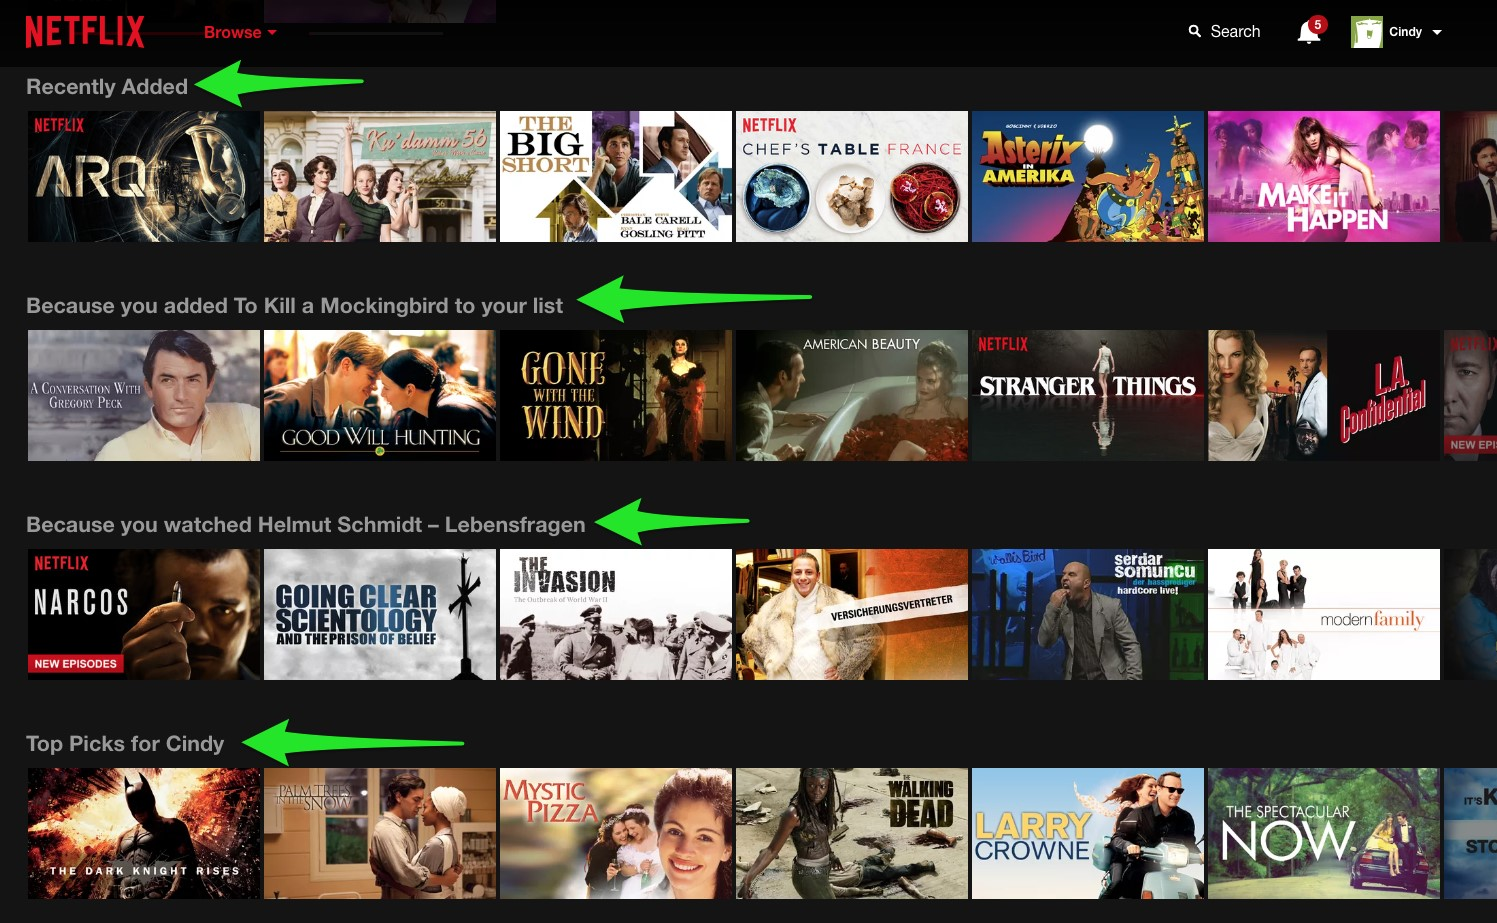
\includegraphics[height=150pt,width=300pt]{img/chapter1/netflix.jpg}
        \caption{Recommandations sur la plate-forme Netflix}
    \end{figure}

\subsubsection*{Système de recommandation pour les articles de presse :} 
\textbf{Google News :} c'est une plate-forme en ligne d'articles de presses obtenues de différentes sources. Initialement Google utilisé un filtrage collaborative, ensuite ils ont combiné l'approche collaborative et l'approche basé contenu pour offrir de meilleurs résultats.\cite{gglnews}


\textbf{Buzzer :} c'est un système de recommandation développé par l'université de Dublin sur la base de nombre de clics limités, ce laboratoire a testé des approches basé sur le public \emph{rank}, \emph{friends rank} et \emph{content rank}. L'évaluation a permis de constater que le nombre de clics le plus important était généré par le \textbf{friends rank}.\cite{gglnews}\\
    \begin{figure}[H]
        \centering
            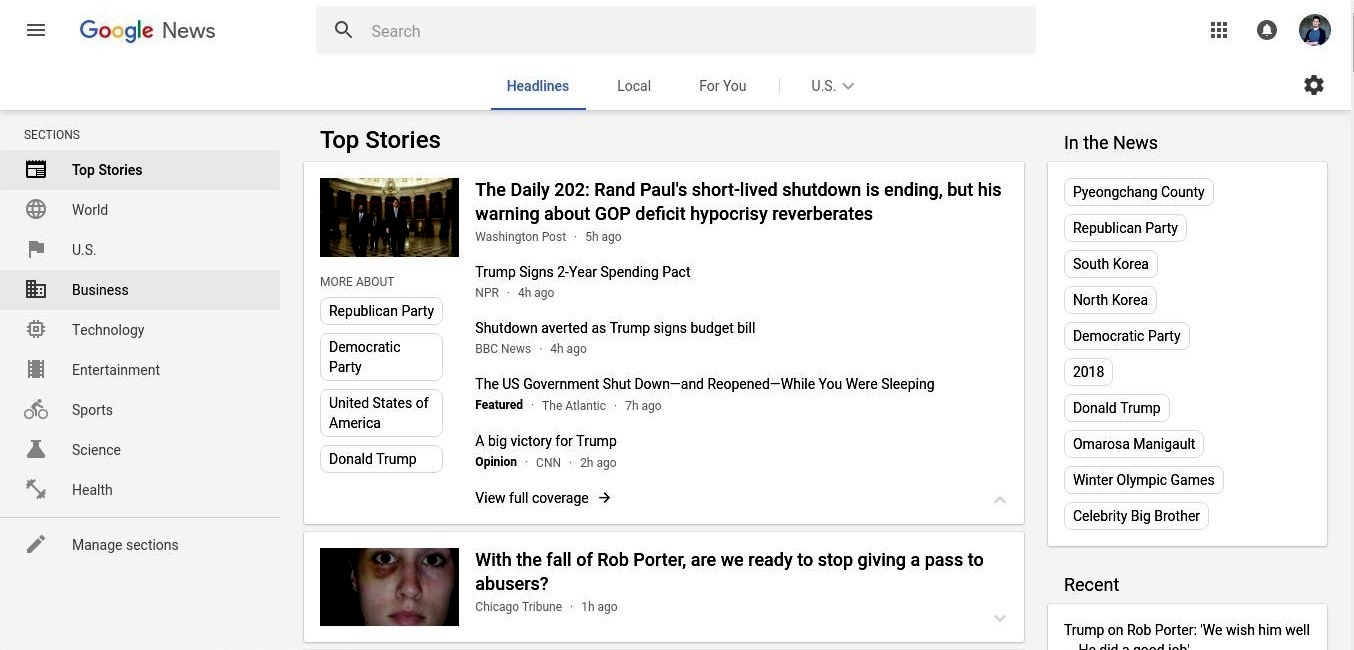
\includegraphics[height=150pt,width=300pt]{img/chapter1/news.jpg}
        \caption{Portail de GoogleNews avec des recommandations}
    \end{figure}

Au terme de ce point, on constate que les systèmes de recommandations participent grandement à promouvoir les objets (produits, multimédia, articles de presse...) puisqu'ils représentent 80\% du contenu proposé, ce qui a diminué des activités des moteurs de recherche de chaque site décrit précédemment puisqu'elles représentent que 20\% des données proposés selon un article intitulé "The Netflix Recommender System:Algorithms,Business Value,and Innovation" apparu sur le site officiel de Netflix.\\

\subsection{Types de systèmes de recommandations}
\begin{figure}[H]
        \centering
            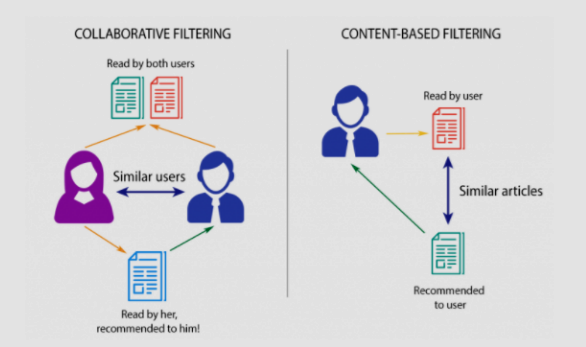
\includegraphics[height=150pt,width=300pt]{img/chapter1/filtering.png}
        \caption{Types de systèmes de recommandations\cite{figfiltering}}

\end{figure}

\begin{itemize}
    \item \textbf{Filtrage basé contenu (Content-based filtering) :\\}
    Une des méthode de recommandation les plus simples, elle consiste à recommander les items ayant le plus de similarité avec les préférences de l'utilisateur.\\

    \item \textbf{Filtrage collaborative (Collaborative filtering) :\\}
    Dans cette approche, la recommandation se fait en utilisant les préférences des profils jugés similaires au profil ciblé, et cela grâce aux préférences précédentes des personnes qui sont regrouper dans des structures de données permettant de calculer la similarité. Parmi les méthodes utilisées on retrouve :
        \begin{enumerate}
            \item \textbf{Memory-based collaborative filtering : }Les notes d'appréciation des utilisateurs sont utilisés pour le calcul de similarité entre utilisateurs ou entre les objets afin de permettre de ciblé au mieux les préférences.\\
            \item \textbf{Model-based collaborative filtering : }Cette technique utilise un modèle de prédiction propre à chaque utilisateur selon les techniques de Datamining, de Recherche d'informations et de Traitement automatique du langage.\\
        \end{enumerate}

    \item \textbf{Filtrage hybride (Hybrid recommender system) :\\}
    Cette approche utilise filtrage basé contenu et filtrage collaborative pour faire face aux problèmes rencontrés en utilisant un filtrage basé contenu seul ou en utilisant un filtrage collaboratif seul. le but est d'avoir une précision maximale mais avec une augmentation de la complexité de calcul.\cite{filtering}
\end{itemize}

\section{Systèmes de recommandations pour les articles de presse}
L'utilisation des systèmes de recommandation pour des sites de vente en ligne ou des réseaux sociaux est très différente à son utilisation pour une revue de presse personnalisé, puisqu'ils y existent des contraintes spécifiques aux revues de presses.
Parmi ces contraintes on retrouve :
\begin{itemize}
    \item \textbf{Cold start : }c'est à dire on possède aucune informations précédentes sur l'utilisateur, ses caractéristiques ou son profil, généralement c'est lors d'une navigation sans identification que ce cas se présente.\\
    \item \textbf{Data sparsity : }les structures de données liées au profil de l'utilisateur peuvent être vide ou très dense ce qui nécessite pour les deux cas un traitement particulier.\\
    \item \textbf{Récence : }dans un système de recommandation traitant des articles de presse, il est inconcevable de proposer d'anciens articles puisque leur importance diminue avec le temps et l'application deviendrait une simple fenêtre à articles ce qui est contraire aux exigences des systèmes de recommandation qui sont de proposer des articles en temps-réel.\\
    \item \textbf{Changement des intérêts des utilisateurs : }c'est la capacité d'adaptation du système de recommandation aux besoins de l'utilisateur, c'est à dire que si ses tendances changent il faut proposer des articles adaptés à ses nouvelles tendances.\\
    \item \textbf{Évolutivité : }C'est la capacité du système à servir plusieurs utilisateurs à la fois et sa rapidité d'interaction avec la source des articles. La dynamique de l'environnement exige une rapidité de calcul en temps réel.\\ 
    \item \textbf{Données non structurés : }les données non-structurés de certaines sources influent sur la capacité du système à recommander des articles.\\
\end{itemize}

\subsection*{Avantages}
L'utilisation des systèmes de recommandations est une approche gagnante sur tout les front que ce soit pour un utilisateur qui trouve tout ce qui cherche de manière facile ou pour l'organisme qui génère à son tour des gains économiques rapidement et efficacement.\\
En effet, les recommandations ciblent directement un article précis pour un utilisateur précis, ce qui va pousser ce dernier à s'accrocher et à continuer ça recherche afin de trouver la meilleure offre possible. D'un autre cote, l'utilisation des profils utilisateurs dans les systèmes de recommandations les rendent beaucoup plus personnalisé et conformes aux besoins réels de l'utilisateur.\cite{figfiltering}

\section{Profilage d'utilisateur}
Dans un monde où l'utilisation des systèmes de recommandation ne cesse d’accroître, la personnalisation d'un objet recommandé devient très importante surtout pour les systèmes basé sur les caractéristiques de chaque profil ou les systèmes hybrides.

\subsection{Définition}
Un profilage est une représentation des intérêts de l'utilisateur sous forme d'une structure de données comportant des informations propres à chaque utilisateur (coordonnés, préférences...) qui peuvent être traiter par des systèmes d'exploitation, des SGBD ou des moteurs de recherches.

\subsection{Contenu du profil utilisateur}
Un profil utilisateur contient des informations qui sont jugées utiles et cela en fonction des besoins, on retrouve par exemple :\\
\begin{itemize}
    \item Un historique qui permet de modéliser les comportement des utilisateurs.
    \item Les centres d’intérêts et les préférences relatives au problème à traité afin de construire un modèle de prédiction pour la recommandation.
\end{itemize}
\textbf{Tout cela, bien sur, en respectant la vie privée des individus et en s'assurant de la sécurité et la confidentialité des données.}

\subsection{Types de profilage d'utilisateurs}
\subsubsection{Profilage explicite (Explicit user profiling)}
Ce type de profil se base uniquement sur les informations fournies par l'utilisateur tel une évaluation d'un objet ou un remplissage de formulaire.\\
Cette approche n'est pas entièrement satisfaisante car la méfiance des utilisateurs (non divulgation des coordonnées, données erronées...) laisse ce type de profilage très dépassé en fonction des besoins.

\subsubsection{Profilage implicite}
Comme l'approche précédente de profilage (le profilage explicite à lui seul) ne donnaient pas suffisamment de bons résultats, l'approche implicite utilise le comportement de l'utilisateur (clics, temps de parcours, historique...).\\
Certes cette méthode réduit l'erreur dans la prédiction mais présente un certain défaut, par exemple, quand un utilisateur achète un produit sur une plate-forme de commerce en ligne pour un ami, cela ne veut en aucun cas dire que l'utilisateur est intéressé par ce produit.

\subsubsection{Profilage hybride}
Ce type de profilage englobe l'approche explicite qui permet de récolter des informations à travers des formulaires et l'approche implicite qui récupère les comportements de l'utilisateur.\\ 
Cette méthode de profilage est plus efficace que les deux précédentes et présente un énorme avantage lors de la recommandation d'informations temporelles (articles de presse).

\subsection{Extraction de profil utilisateur}
L'extraction du profil utilisateur représente une étape clé dans le processus de profilage, elle peut se faire de manière générale par extraction des données (Amis, contenu partagé, coordonnées...) à partir des sites web, des réseaux sociaux ou des plate-formes de e-commerce.\\ 
Néanmoins ceci ne suffit pas dans tous les cas, faute de précision de la ciblage. Une autre approche a été introduite pour l'extraction des profils par Yoshinori Hijikata qui a fait une étude sur l'extraction de profil suivant le mouvement de la souris de l'ordinateur, on peut cités quelques un:
\begin{itemize}
    \item Suivi de texte: le déplacement du pointeur de la souris le long d'une phrase pendant la lecture.
    \item Pointage de lien: positionnement du pointeur de la souris sur un lien sans forcément cliquer dessus.
    \item Clique sur un lien: en cliquant sur un lien pour passer à une autre page.
    \item Sélection de texte: sélection du texte en faisant glisser le pointeur de la souris.
    \item Défilement: vitesse de défilement d'une fenêtre.
    \item Enregistrement de signets: enregistrement d'une page en tant que signet.
    \item Enregistrement d'une page : enregistrement d'un document HTML.
    \item Impression: impression d'une page.
    \item Déplacement de la fenêtre: déplacement d'une fenêtre du navigateur Web.
    \item Redimensionnement de la fenêtre: modification de la taille de la fenêtre du navigateur Web.
    \item TimeOnMouse: nombre de millisecondes passées par l'utilisateur lors du déplacement de la souris.
    \item TimeOnPage: nombre de millisecondes passées par l'utilisateur sur une page ou un article de news.
    \item EventOnScroll: nombre de clics dans les barres de défilement.
    \item ClickOnWindow: nombre de clics dans la fenêtre du navigateur mais pas dans les barres de défilement.
    \item TimeOnH/VScroll: nombre de millisecondes passées par l'utilisateur à utiliser le défilement horizontal ou vertical.
    \item NumOfPageUp/Down: nombre de pages que l'utilisateur a fait défiler vers le haut ou bas.
    \item MSecForPageUp/Down: nombre de millisecondes passées par l'utilisateur à faire défiler une page.
    \item NumOfUp/DownArrow: nombre de clics sur la touche fléchée vers le haut ou bas.
    \item MSecForUp/DownArrow: nombre de millisecondes passées par l'utilisateur sur la touche fléchée vers le haut ou bas.\cite{profil}
\end{itemize}

\begin{figure}[H]
\begin{lstlisting}[style=code]
    {
    "_id" : "251850BE-DFF5-4AAB-A12D-98D4A4606028" ,
    "articleid" : "318218311" ,
    "userid" : "bf4d2584fd66a214bcf" ,
    "eventType" : "TIME_SPENT_ARTICLE_VIEW" ,
    "timestamp" : {"$date" : "2013-06-12T16:41:15.5125"} ,
    "geolocation" : { "name" : " " ,
                    "type" : " " ,
                    "longitude" : 8.00354 ,
                    "latitude" : 58.138821 } ,
    "properties" : {"duration" : "1.427272"} ,
    "tags" : [ "agder politidistrikt", "havnet", "satt", "rebelksmannen", "operajonsleder", "kristiansund slo", "politiet", "kristiansand skalled", "Maharashtra", "india", "Egersund", "Rogaland", "Norway"] ,
    "categories" : ["NEWS"]}
\end{lstlisting}
\caption{Exemple d'un profil utilisateur}
\end{figure}

\section{Conclusion}
Vu l'importance des systèmes de recommandations aujourd'hui, leurs places est plus que jamais primordiale à l'élaboration d'une application intelligente capable de traiter des informations en temps réel et de les fournir de manière personnalisée aux utilisateurs.\\
Durant ce chapitre, nous avons commencé par présenter les différentes approches de l'apprentissage automatique, ensuite nous avons détaillé ce qu'est un système de recommandation, ses types et un bref état de l'art sur les systèmes les plus utilisés couramment et leurs avantages.\\ 
Enfin, nous avons expliqué la notion de profil d'utilisateur, ses types et son extraction. Dans le chapitre suivant, il en sera question de faire une introduction au traitement automatique du langage et de traiter ses différents aspects.